\documentclass[11pt, oneside]{article}   	% use "amsart" instead of "article" for AMSLaTeX format
\usepackage{geometry}                		% See geometry.pdf to learn the layout options. There are lots.
\geometry{letterpaper}                   		% ... or a4paper or a5paper or ... 
%\geometry{landscape}                		% Activate for for rotated page geometry
%\usepackage[parfill]{parskip}    		% Activate to begin paragraphs with an empty line rather than an indent
\usepackage{graphicx}				% Use pdf, png, jpg, or eps� with pdflatex; use eps in DVI mode
								% TeX will automatically convert eps --> pdf in pdflatex		
\usepackage{amssymb}

\usepackage{amsmath}

\title{HomeActivity: Recognizing home activities using sensor data}
\author{Stephen Lee, Patrick Pagus and Dong Chen\\ 
ML Final Project}
%\date{}							% Activate to display a given date or no date

\begin{document}
\maketitle
%\section{}
%\subsection{}
\section{Abstract:}

In this project, we user sensors deployed in homes to identify activities. The actuation of sensors provides a unique set of feature representation that allows us to identity 
the type of activity being undertaken by the user. The goal of our project is to use these sensor information to infer activities under different methodologies and analyze their 
performance.  We use datasets from three different houses that are annotated manually to get the 'ground truth'.  To capture the underlying model, we use different feature representations from the sensors. We present our results and discuss our findings. 
 

%Recognizing home activities allows many potential smart applications including healthcare and energy efficiency. In this project, we present the state of the art models for recognizing activities, and show how they performance on the Kasteren-a real world dataset. 
%Comparative analysis metrics including precision, recall, accuracy, F1 mesure and MCC are used in the experiments. Our evaluation results could be used for other pattern recognizing area rather than home activity recognizing.

\section{Introduction}
According to a recent study,  it is estimated that almost 25+ billion Internet of Things (IoT) devices will be deployed across homes. Moreover, around 50 trillion GBs of 
data will be collected using these sensors. The information collected can be used to enrich the interaction between users and the physical devices. For example, NEST thermostat, 
an intelligent programmable thermostat, learns the occupancy of humans in a home using sensors to automatically turn on/off heating or air conditioning and save energy costs. These sensor information can be used to learn other information such as monitoring the activities of a person (e.g. elderly home) and being able to detect anomalies in behavior over time. In this project, we focus on recognizing the activities of a person using the sensor information available. i.e. We study different techniques to identify when the person is sleeping, eating etc. 

Activity recognition has been a widely studied area and provides a set of challenges in itself. First, ambiguity exists if there are more than one activity happening concurrently at any given time, such as watching TV and eating a snack. Also, this muddles the distinction between the start and end of an activity. Second, activation of a sensor may represent doing a similar activity. For example, opening the fridge could represent 'getting a snack' activity or 'cooking' activity'. Third, the information could be noisy e.g. with misfiring sensors or a mistakes made by humans such as unintentionally opening a cupboard or entering a room. Fourth, recognizing activities has class imbalance as certain activity labels tend to be longer than others. For example, lying on bed or couch, staying idle, or 'not at home' could easily represent the dominant classes in these datasets. 

Clearly, activity recognition is a challenging problem. Thus, we chose a dataset wherein the homes was occupied by a single user. We construct features using the binary sensors installed in these homes that we will describe later in section. In fact, we construct multiple feature representations to study the problem and follow closely the approaches studied by Kasteren~\cite{tvkasteren} among others. In the following section, we will be describing our approach, and discuss its performance and lessons learned from undertaking this project.


%Automatically recognizing human activities such as cooking, sleeping and bathing, in a home setting allows many applications in areas such as intelligent environments and 
%healthcare. In healthcare, home activity recognition can be used to assess the cognitive and physical capabilities of an elderly person. Home energy efficiency can be improved given 
%a schedule of the occupant's activities by scheduling background loads, such as heating, cooling, and various appliances. 

%Recent developments in sensing technology has led to wireless sensor networks which provide a non-intrusive, privacy friendly and easy to install solution to in-home monitoring. 
%Sensors used are contact switches to measure open-close states of do	ors and cupboards; pressure mats to measure sitting on a couch or lying in bed; mercury contacts for 
%movement of objects such as drawers; passive infrared sensors to detect motion in a specific area and float sensors to measure the toilet being flushed. 
%More formally, activity recognition finds a function that maps a sequence of sensor readings (feature vectors), to a sequence of activity labels that best describes the sensor data. We 
%focus on activity recognition within home based wireless sensor networks. This domain has several challenges. First, there is a dearth of training data because labeling one's activities 
%is a tedious time consuming process, this limits the number of effective techniques. Second, patterns in training data are specific to the home and the individual. Therefore, the 
%performance of the different machine learning technique may vary widely over a real world dataset. Finally, dominant classes may confound machine learning techniques.

%To further our knowledge of machine learning, we will conduct a comprehensive empirical analysis of proposed methods in this domain. These methods include Hidden Markov Models(HMM), Conditional Random Fields(CRF), Support Vector Machines(SVM), and Structured Support Vector Machines(SSVM) and Naive Bayes (NB). We implemented the models in Python and apply these methods to Kasteren-a real world dataset. By applying these techniques to real-world datasets and explaining the differences and similarities in their performances, we will gain a deeper understanding of machine learning. Furthermore, 
%Our evaluation results could be used as a baseline for other pattern recognizing area rather than home activity recognizing.
\section{Related Work}\label{sec:related}

Home occupant activities recognition problem has been studied for several years. There is inherent challenge in collecting accurate data from homes for research purposes. In~\cite{emtapia}, Tapia et al. deployed low-cost sensors to monitor occupant activities at home. As reported, using this sensor information, they can detect events of interest to healthcare professionals, such as toileting and bathing, in real residential places with accuracy ranging from 25\% to 89\%. 
We follow closely the work of the of Kasteren et. al. ~\cite{tvkasteren,tvkasteren2010}, and use their datasets for our evaluation. In their evaluation, they use Naive Bayes, HMM, and CRF to evaluate activity recognition using the sensor readings deployed in their homes. In our approach, we evaluated the dataset on a wider range of models. 

%In ~\cite{djpatt}, Patterson et al. collected object data using a glove outfitted with a Radio Frequency Identification (RFID) antenna. They used three models, including training HMMs separately, coupling HMMs into a one large system and using execution history of those objects, to recognize object-interaction based activity in a more realistic setting. They found that utilizing object history has the best accuracy-81.2\%. 

%In~\cite{tvkasteren}, Kasteren et al. designed  wireless sensor network (WSN) and a low-cost but discrete annotation method to automatically recognize activities. They use Raw, Changepoint, and Last methods are employed to represent sensor information, which forms the basis of our feature representations. Their approach uses HMM and CRF models for recognizing activities but do not use models such as structured support vector machines to evaluate. 

%In~\cite{tduong}, Duong et al. argue that instead of only using duration pattern, it would be more beneficial to combine inherent hierarchical structures. A switching hidden semi-Markov model is used to empirically compare performance with traditional models. Interestingly, the experiments are tested on a tracking missing and activities overlapping dataset. In~\cite{sluhr}, Sebastian et al. point out the Hierarchical Hidden Markov Model can capture the natural hierarchy information presentation in home activities when generating models. As shown, they are able to learn two simple activity sequences and capture the hierarchical structure represented in the data. In~\cite{noliver}, Oliver et al. use a Layered Hidden Markov Models to infer user activity status from online stream data (e.g. video, autio, keyboard and mouse clicks). Using this cascade of HMMs, they can do sensing, training and predicting at different office data granularity. In~\cite{asubr}, Subramanya et al. design a hierarchical model in order to monitoring the motion status and context status for a real person. As shown in the work, breaking a big complex activity into smaller sub-activities to build models is very useful for recognizing person activities. Our project follows closely the approaches presented by Kasteren in work~\cite{tvkasteren}  others. We describe the work undertaken and highlight our findings, issues and limitations that are still required to be overcome in this report.


\section{Approach}

We explore and implement the following techniques to recognize activities:
%Inferring and recognizing occupant activities using sensors home deployed sensors requires us to solve the following issues. 
%
%First, the start and end time of a performed activity is unknown. When activities are performed around the house there is no clear indication when one activity ends and another one starts. 
%
%Second, there is ambiguity in the observed sensor data with respect to which activity is taking place. For example, cooking and getting a drink both involve opening the fridge. Sensors can measure that the fridge is opened, but not which item is taken from the fridge. 
%
%Third, activities can be performed in a large number of ways, making it difficult to create a general description of an activity. 
%
%Fourth, observed sensor data is noisy. Noise can either be caused by a human making a mistake, for example opening a wrong cupboard, or by the sensor system which fails to transmit a sensor reading due to a network glitch.
%
%These issues make activity recognition a very challenging task. 
%
%Many different models have been proposed for activity recognition, but no common benchmark for evaluating the performance of these models exists. In this project we implenent the state of the art probabilistic models used in activity recognition and show their performance on several real world datasets. Our results can be used as a baseline for comparing the performance of other pattern recognition methods (both probabilistic and non-probabilistic). 


\subsection{Hidden Markov Models (HMM)}
HMM is a generative probabilistic model that models the joint distribution of both the observed and the latent states. It is commonly used in recognizing temporal patterns such as handwriting and speech recognition, where the future state is dependent on the previous state.  In our project, the latent variable($\bf{y}$) is the activity performed by the user, and the observed variable($\bf{x}$) is the vector of sensor readings. 

At each time step $t$, the latent variable $y_t$ depends only on the previous hidden variable $y_{t-1}$ and variables before $t-1$have no influence on it (Markov Property). The observed variable $x_t$, at time $t$, depends only on the latent variable $y_t$. The parameters of the HMM model are the transition probabilities $p(y_{t}\mid y_{t-1})$ i.e.  the probability of going from one state to another; and the emission probability $p(x_{t}\mid y_{t})$ i.e. the probability that the state $y_t$ would generate observation $x_{t}$. In order to learn the parameters of the distribution, one can maximize the joint probability $P(x,y)$ of the observed and latent sequences in the training data. The joint probability can be factorized as follows:

%There are two dependency assumptions: The hidden variable at time t, namely $y_{t}$, depends only on the previous hidden variable $y_{t-1}$. The observable variable at time t, namely $x_{t}$, depends only on the hidden variable $y_{t}$ at that time slice. Then, we can specify an HMM using three probability distributions: the distribution over initial states p($y_{1}$); the transition distribution $p(y_{t}\mid y_{t-1})$ representing the probability of going from one state to the next; and the observation distribution $p(x_{t}\mid y_{t})$ indicating the probability that the state yt would generate observation $x_{t}$.
%Learning the parameters of these distributions corresponds to maximizing the joint probability p(x, y) of the paired observation and label sequences in the training data. We can factorize the joint distribution in terms of the three distributions described above as follows:

\begin{equation}
P(x,y)=\prod_{t=1}^{T}p(y_{t}\mid y_{t-1})p(x_{t}\mid y_{t}), p(y_{1}) = p(y_{1}\mid y_{0})
\end{equation}

Since the data is discrete in nature, frequency counting can be used to learn the parameters. We use Viterbi algorithm to infer the sequence of activity labels from the observed sensor reading sequences. 

\subsection{Conditional Random Fields (CRF)}
We use linear-chain CRF to represent the latent and observed variables as it closely resembles the HMM in terms of structure. Since, CRF is a discriminative probabilistic model, we can model the conditional probability distribution $P(y \mid x)$, to predict $y$ from $x$. Thus, the parameters are learnt by maximizing the following  conditional probability distribution $P(y \mid x)$,
%We define the linear-chain CRF as a discriminative analog of the previously defined HMM, so that the conditional distribution is defined as
\begin{equation}
p(y\mid x)=\frac{1}{Z(x)}exp\left[{\sum_{k=1}^{K}}{\lambda}_{k}{f}_{k}({y}_{t},{y}_{t-1},{x}_{t})\right]
\end{equation}
where \textit{K} is the number of feature functions used to parameterize the distribution, ${\lambda}_{k}$ is the weight parameter and ${f}_{k}({y}_{t},{y}_{t-1},{x}_{t})$ is a feature function. 
The product of the parameters and the feature function ${\lambda}_{k}{f}_{k}({y}_{t},{y}_{t-1},{x}_{t})$ is called the energy function, while the exponential representation is the potential function. The partition function \textit{Z(x)} is a normalization constant that sums over all the potential functions and is given as follows:

%where \textit{K} is the number of feature functions used to parameterize the distribution, ${\lambda}_{k}$ is the weight parameter and ${f}_{k}({y}_{t},{y}_{t-1},{x}_{t})$ is the feather function. The product of the parameters and the feature function${\lambda}_{k}{f}_{k}({y}_{t},{y}_{t-1},{x}_{t})$ is called energy function, while the exponential representation is the potential function. The partiton function \textit{Z(x)} is normalization term in order to make the distribution sums up to one and obtains a probabilistic interpretation.

\begin{equation}
Z(x)=\sum_{y}^{}exp\left[{\sum_{k=1}^{K}}{\lambda}_{k}{f}_{k}({y}_{t},{y}_{t-1},{x}_{t})\right]
\end{equation}

In our approach, we use the BFGS method to learn the parameters of the model. 

\subsection{Support Vector Machines (SVM)}  
SVM is a discriminative classifier that builds a hyperplane that can be used for classification or regression purposes. It constructs this hyperplane such that 
the distance between the hyperplane and the nearest point is maximized.  In particular, the problem can be seen as minimizing a loss function that can be represented as following:

\begin{align*}
\min_{w, \beta} L(w) = \frac{1}{2}||w||^{2} \\ 
\text{ subject to } y_{i}(w^{T} x_{i} + \beta) \geq 1 \text{ } \forall i,
\end{align*}
where $x_i$ are the training examples, $y_i$ represent the labels, $w$ represents the weight vector and $\beta$ is the bias. In our approach, we use
a Linear SVM for classification.
 
\subsection{Structured Support Vector Machines (SSVM)}
Structured SVM, as the name suggests, makes use of the structure of the output space for classification purposes. It is generally used for classification where the goal is to predict a sequence as compared to a single label in SVM. The loss function is represented by

\begin{equation}
y^* = \arg \max_{y \in Y} g(x, y)
\end{equation}
where $x$ is the input, $Y$ is the set of all possible output and $g$ is the loss function given by,
\begin{equation}
g(x, y) = w^T f(x, y)
\end{equation}
Here, the $f$ is feature function, and we use the linear chain CRF model to represent the feature function i.e. the linear combination of the feature potential(nodes) and the transition potential (edges). The parameters of $g(x,y)$ is learnt by minimizing a loss. We use the libraries provided in \emph{pystruct} for classifying the input variables.

\subsection{Naive Bayes}
The naive Bayes model is one of the most simplistic probabilistic models. Unlike the other models, the naive Bayes model assumes all data points are independently and identically distributed (i.i.d.), that is it does not take into account any temporal relations between data points. The model factorizes the joint probability over the datapoints as follows,
\begin{equation}
p({y}_{1:T},{x}_{1:T})=\prod_{t=1}^{T}p({{x}_{t}\mid {y}_{t}}^{})p({y}_{t})
\end{equation}
we apply the naive Bayes assumption, which means we model each sensor reading separately, requiring only
\textit{N} parameters for each activity. The observation distribution therefore factorizes as
\begin{equation}
p({x}_{t}\mid{y}_{t}=i)=\prod_{n=1}^{N}p({{x}_{t}^{n}\mid {y}_{t}}=i)
\end{equation}
where each sensor observation is modeled as an independent Bernoulli distribution, given by
\begin{equation}
p({{x}_{t}^{n}\mid {y}_{t}}=i)={{\mu}_{ni}}^{{{x}_{t}}^n}{(1-{\mu}_{ni})}^{1-{{x}_{t}}^n}
\end{equation}


\iffalse
The datasets available to us are:
	\begin{enumerate}
\item Kasteren dataset - has over a month long sensor information from 3 homes.
\item Tulum dataset - more than six month period from a single home
	\end{enumerate}
\fi

\subsection{Experimental Setup}

We use http://scikit-learn.org packages to present the models.



\subsection{Feather Representation}

Raw: the raw sensor representation uses the sensor data directly as it was received from the sensors. It gives a 1 when the sensor is firing and a 0 otherwise 


Change: The change point representation indicates when a sensor event takes place. That is, it indicates when a sensor changes value. More formally, it gives a 1 when a sensor changes state (i.e. goes from zero to one or vice versa) and a 0 otherwise.

Last: The last-fired sensor representation indicates which sensor fired last. The sen- sor that changed state last continues to give 1 and changes to 0 when another sensor changes state 

5 fold – cross validation

Divide the dataset into smaller subsequences of ~2 hours 



\section{Experimental Evaluation}

\subsection{Datasets}

The Kasteren dataset is recording a 26-year-old man. He lives alone in a three-room apartment where 14 state-change sensors were installed. Locations of sensors include doors, cup- boards, refrigerator and a toilet flush sensor. Sensors were left unattended, collecting data for 28 days in the apartment. This resulted in 2120 sensor events and 245 activity instances.

As shown in the table, for Kasteren dataset we have three houses with 14, 23, 21 sensors, respectively.

The tableis an example of referenced \LaTeX elements.
 
\begin{table*}[t!]
\small
\begin{center}
\begin{tabular}{||c|c|c|c|||}
\hline
\textbf{Type} & \emph{House A} & \emph{House B} & \emph{House C}\\ \hline
\textbf{Age} & 26 & 28 & 27\\ \hline
\textbf{Gender} & M & M & M\\ \hline
\textbf{Setting} & Apartment & Apartment & House\\ \hline
\textbf{Room} & 3 & 2 & 6\\ \hline
\textbf{Duration(days)} & 25 & 14 & 19\\ \hline
\textbf{Sensors} & 14 & 23 & 21\\ \hline
\textbf{Activities} & 10 & 13 & 16\\ \hline
\textbf{Annotation} & Bluetooth & Diary & Bluetooh\\ \hline
\end{tabular}
\end{center}
%\vspace{-0.1cm}
\caption{Dataset recording details}
\label{table:fake-attacks}
\vspace{-0.3cm}
\end{table*}




\subsection{Comparative Analysis Metrics}

\begin{equation}
Precision = \frac{TP}{TP+FP}
\end{equation}

\begin{equation}
Recall = \frac{TP}{TP+FN}
\end{equation}

\begin{equation}
Accuracy = \frac{TP+TN}{TP+TN+FP+FN}
\end{equation}

\begin{equation}
F-Measure = \frac{2\cdot Precision\cdot Recall}{Precison+Recall}
\end{equation}

The Matthews correlation coefficient is used in machine learning as a measure of the quality of binary (two-class) classifications, introduced by biochemist Brian W. Matthews in 1975. It takes into account true and false positives and negatives and is generally regarded as a balanced measure which can be used even if the classes are of very different sizes. The MCC is in essence a correlation coefficient between the observed and predicted binary classifications; it returns a value between ‚àí1 and +1. A coefficient of +1 represents a perfect prediction, 0 no better than random prediction and ‚àí1 indicates total disagreement between prediction and observation.

\begin{equation}
MCC=\frac{TP\cdot TN-FP\cdot FN}{\sqrt{(TP+FP)\cdot (TP+FN)\cdot (TN+FP)\cdot (TN+FN)}}
\end{equation}


\subsection{Experiments}
%\pdfsuppresswarningpagegroup=1
\begin{figure}[t!]
\begin{center}
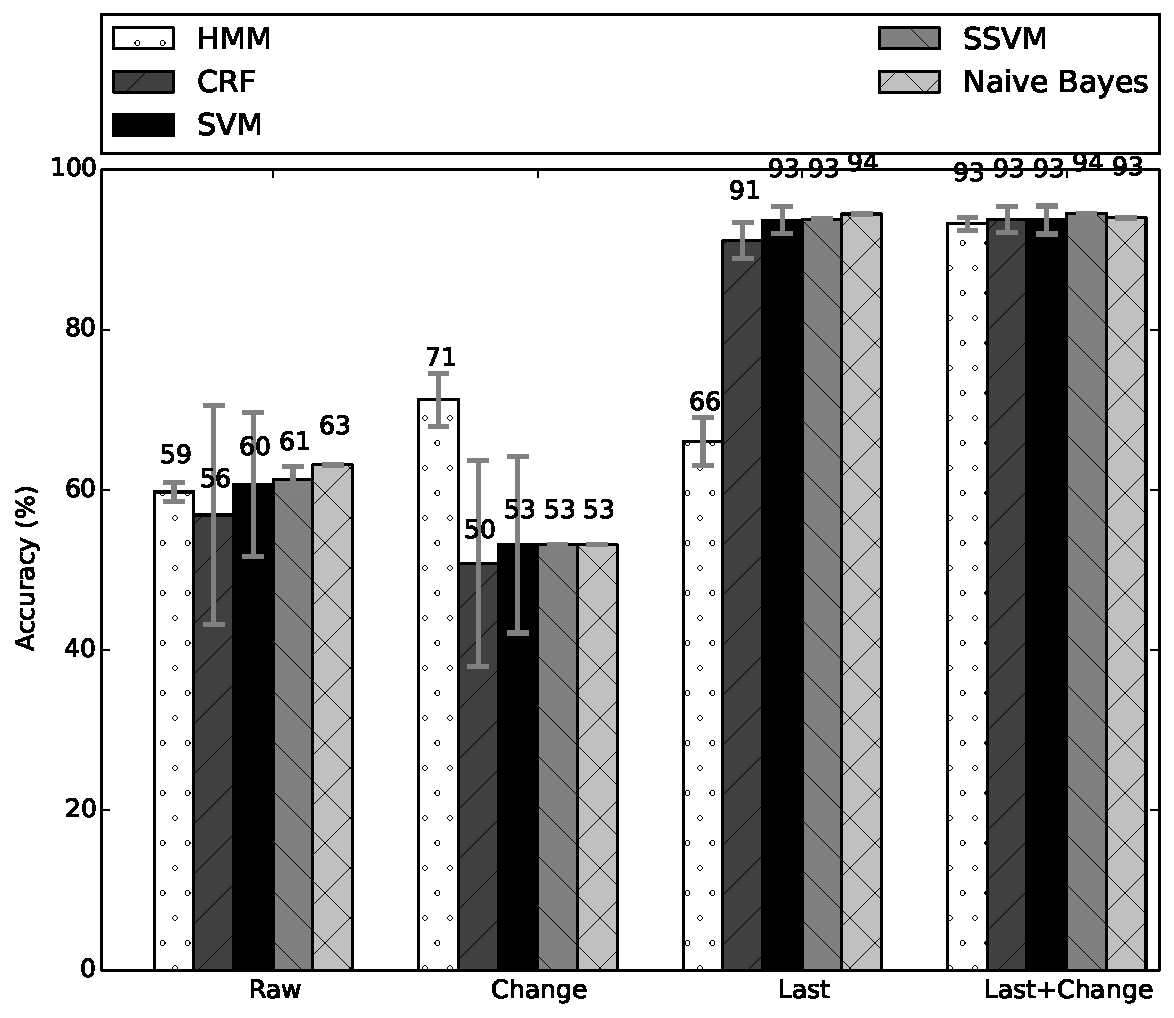
\includegraphics[width=5in]{../../src/reports/A.pdf}
\end{center}
\vspace{-0.5cm}
\caption{House A}
\label{fig:house_a}
\vspace{-0.5cm}
\end{figure}

\begin{figure}[t!]
\begin{center}
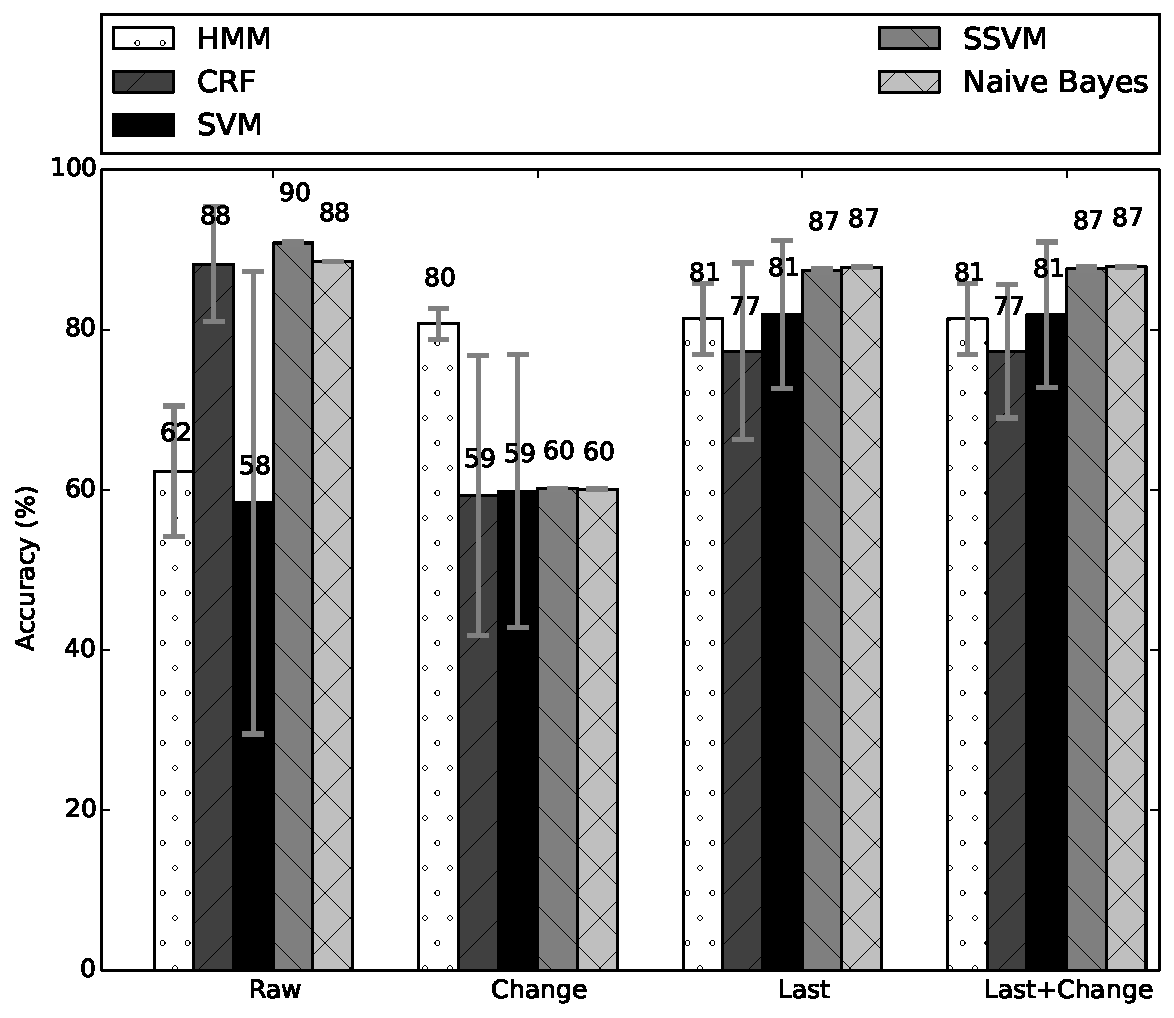
\includegraphics[width=5in]{../../src/reports/B.pdf}
\end{center}
\vspace{-0.5cm}
\caption{House B}
\label{fig:house_b}
\vspace{-0.5cm}
\end{figure}

\begin{figure}[t!]
\begin{center}
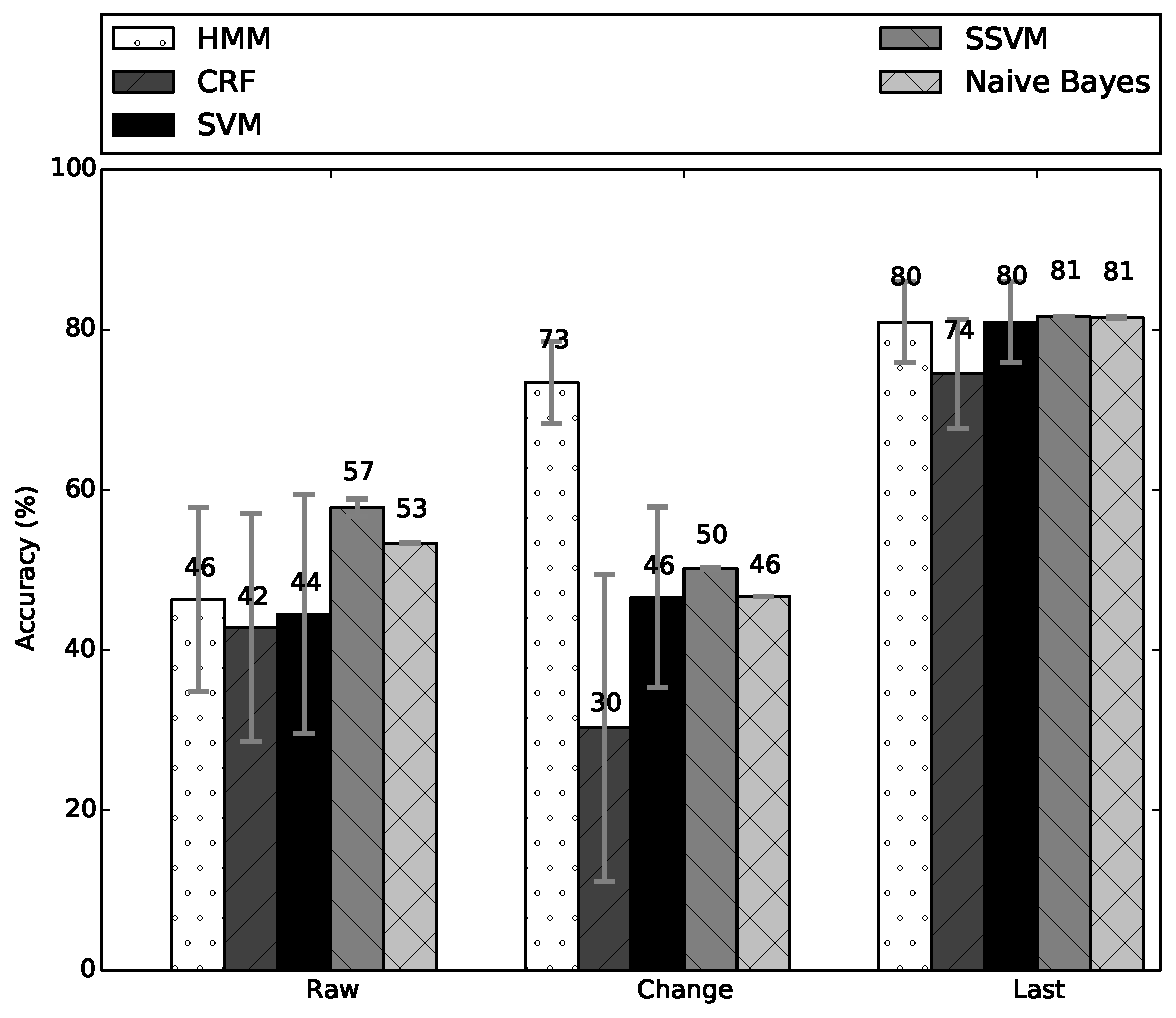
\includegraphics[width=5in]{../../src/reports/C.pdf}
\end{center}
\vspace{-0.5cm}
\caption{House C}
\label{fig:house_3}
\vspace{-0.5cm}
\end{figure}





\section{Conclusions and Lessons Learned}


%\section{Reference}

\begin{thebibliography}{1}
	
\bibitem{emtapia} E. M. Tapia, S. S. Intille, and K. Larson. {\em Activity recognition in the home using simple and ubiquitous sensors}. In Pervasive Computing, Second International Conference, PERVASIVE 2004, pp. 158–175, Vienna, Austria (April, 2004).

\bibitem{djpatt}  D. J. Patterson, D. Fox, H. A. Kautz, and M. Philipose. Fine-grained activity recognition by aggregating abstract object usage. In ISWC, pp. 44–51. IEEE Computer Society, (2005). ISBN 0-7695-2419-2. URL http://doi.ieeecomputersociety.org/10.1109/ISWC.2005.22.

\bibitem{tvkasteren}  T. van Kasteren, A. Noulas, G. Englebienne, and B. Kro ̈se. Accurate activity recognition in a home setting. In UbiComp ’08: Proceedings of the 10th international conference on Ubiquitous computing, pp. 1–9, New York, NY, USA, (2008). ACM. ISBN 978-1-60558-136-1. doi: http: //doi.acm.org/10.1145/1409635.1409637.

\bibitem{tduong}  T. Duong, D. Phung, H. Bui, and S. Venkatesh, Efficient duration and hierarchical modeling for human activity recognition, Artif. Intell. 173(7-8), 830–856, (2009). ISSN 0004-3702. doi: http://dx.doi.org/10.1016/j.artint.2008.12.005.

\bibitem{sluhr}  S. Luhr, H. H. Bui, S. Venkatesh, and G. A. West, Recognition of human activity through hierarchical stochastic learning, percom. 00, 416, (2003). doi: http://doi.ieeecomputersociety. org/10.1109/PERCOM.2003.1192766.

\bibitem{noliver}  N. Oliver, A. Garg, and E. Horvitz, Layered representations for learning and inferring office activity from multiple sensory channels, Comput. Vis. Image Underst. 96(2), 163–180, (2004). ISSN 1077-3142. doi: http://dx.doi.org/10.1016/j.cviu.2004.02.004.

\bibitem{asubr}  A. Subramanya, A. Raj, J. Bilmes, and D. Fox. Hierarchical models for activity recognition. In IEEE Multimedia Signal Processing (MMSP) Conference, Victoria, CA (October, 2006).


\end{thebibliography}

\end{document}  


\begin{enumerate}
 
\item Interesting because it has applications that spans across various domains:
	\begin{enumerate}
	\item Healthcare\\
		- Long term monitoring of activities could provide us interesting insights on degenerative heath \\
		- Especially useful in monitoring health of elderly people\\
	\item  Energy savings \\
		- Understanding the pattern of activities could help us save energy. \\
		- For example, switching off AC/heater when no one is at home \\
	\item  From a Security perspective\\
		- Again, notifications can be sent to alert the home owners if there is an aberrant activity in the door entrance. \\
	\item  Intelligent Homes\\
		- 
	\end{enumerate}
\item Challenging
		\begin{enumerate}
	\item Sensor datasets could be noisy\\
		- the front doors may open and close multiple times; this doesn't may not indicate that the person has left the home.\\
		- sometimes the sensors itself may have false positives. \\
		
	\item multiple labels may be mapped to a single sensor activity\\
		- opening of a fridge may mean both; make coffee and make cooking\\
		- some other information such as how long the person spent in the kitchen may provide some useful insight\\
		
	\item Imbalanced class problem\\
		- machine learning algorithms and works best when the number of instances of each classes are roughly equal\\
		- where the total number of a class of data (positive) is far less than the total number of another class of data (negative)	\\
		- In this problem, no activity is a perfectly reasonable label. So the prediction model may always output 'no activity' and be accurate 80\% of the time.\\
		\end{enumerate}

\end{enumerate}
